\section{Preparazione dei modelli}

La preparazione dei modelli costituisce un passaggio fondamentale nella pipeline di animazione 3D, poiché determina sia la struttura geometrica degli oggetti sia la configurazione dello scheletro necessario per il loro movimento. In questo capitolo, si descrive il processo seguito per la creazione di modelli modulari e per la generazione automatica di un rigging iniziale utilizzando \textbf{Blender} come ambiente di lavoro principale.

L'obiettivo di questa fase è duplice: da un lato, garantire che le mesh siano organizzate e pronte per essere animate; dall'altro, creare uno scheletro coerente e funzionale, in grado di supportare deformazioni realistiche e di integrarsi con animazioni predefinite. Per facilitare questo processo, sono stati impiegati riferimenti a scheletri umanoidi standard, adattati alle specificità dei modelli utilizzati.

\subsection{Descrizione della mesh}

La fase di definizione delle mesh costituiscce il primo passo nella preparazione dei modelli per l'animazione in Blender. In questo lavoro, i modelli sono stati realizzati in forma modulare, al fine di consentire una gestione semplice e flessibile delle diverse componenti durante la fase di rigging, skinning e animazione.

I modelli principali utilizzati sono i seguenti: 
\begin{itemize}
    \item \textbf{Piatto con gambe}: rappresenta una struttura base costituita da una mesh piana (piatto) che funge da corpo principale, integrata con due gambe posizionate simmetricamente per consentire il movimento verticale e traslatorio. Questa configurazione permette di testare deformazioni e animazioni di base come camminata o rotazioni.
    \item \textbf{Piattino con tazzina e gambe}: questa combinazione rappresenta una forma più complessa, in cui la tazzina è posizionata sopra il piattino, entrambi supportati da due gambe. Tale struttura offre un maggiore livello di articolazione e permette di sperimentare il comportamento delle mesh durante animazioni più complesse, simulando un personaggio modulare con elementi sovrapposti.
\end{itemize}

Ogni mesh è stata importata in Blender come oggetto separato, con una propria origine e pivot point, per facilitare l'allineamento con lo scheletro e garantire una corretta deformazione durante l'animazione. L'approccio modulare consente inoltre di sostituire o modificare singoli componenti senza compromettere l'intera struttura del modello.

\begin{figure}[h]
\centering
\begin{subfigure}{0.45\textwidth}
    \centering
    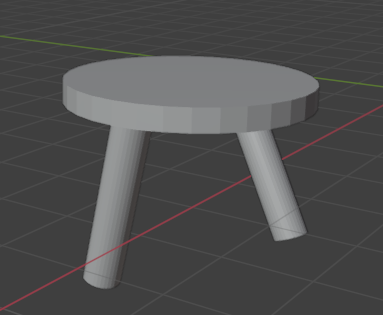
\includegraphics[width=\linewidth]{figure/piatto.png}
    \caption{Piatto con gambe}
\end{subfigure}
\hfill
\begin{subfigure}{0.45\textwidth}
    \centering
    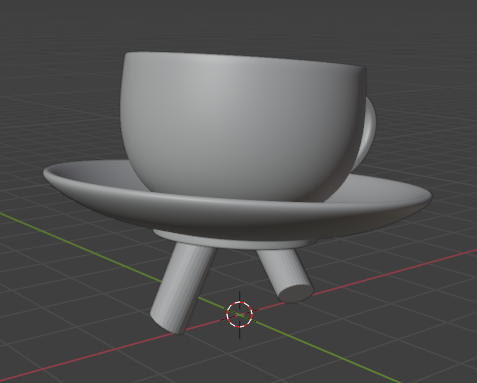
\includegraphics[width=\linewidth]{figure/tazza.png}
    \caption{Piattino con tazzina e gambe}
\end{subfigure}
\caption{Mesh dei modelli in Blender}
\end{figure}

\subsection{Creazione dello scheletro iniziale (da rig umanoide)}

La definizione dello scheletro iniziale rappresenta il passaggio fondamentale per consentire l'animazione di un modello. Lo \textbf{scheletro}, o \textit{rig}, è costituito da una struttura gerarchica (Figura ~\ref{fig:gera}) di ossa che permette la deformazione controllata delle mesh durante il movimento. La scelta di utilizzare un \textbf{rig umanoide come riferimento}, come si evidenza in figura ~\ref{fig:scheletro}, deriva dalla necessità di disporre di una struttura articolare coerente, facilmente adattabile a modelli anche non antropomorfi.

\begin{figure}[h]
\begin{center}
     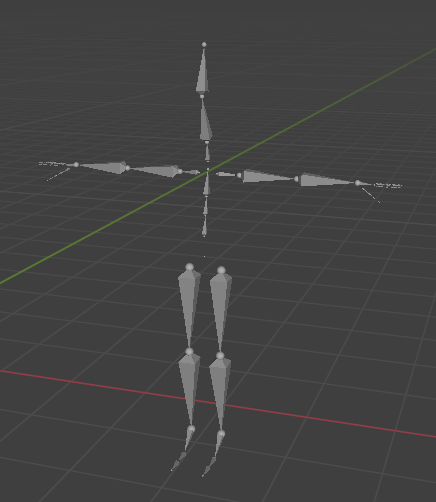
\includegraphics[width=8cm]{figure/scheletro.png}
     \caption{Struttura gerarchica} \label{fig:scheletro}
\end{center}
\end{figure}

Un rig umanoide standard generalmente composto da elementi ricorrenti, quali:
\begin{itemize}
    \item una colonna strutturale centrale (spina dorsale);
    \item due arti inferiori con articolazione dell'anca, del ginocchio e della caviglia;
    \item due arti superiori con articolazione della spalla, del gomito e del polso;
    \item un nodo centrale di orientamento (pelvis o root).
\end{itemize}

Sebbene i modelli trattati in questo lavoro non riproducano figure umane, la \textbf{logica articolare umanoide} risulta comunque utile. Le "gambe" dei modelli, infatti, devono essere in grado di simulare movimenti come passo, flessione o rotazione, che trovano un riferimento diretto nelle articolazioni del corpo umano.

\begin{figure}[h]
\begin{center}
     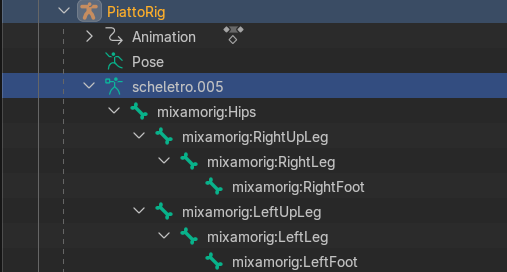
\includegraphics[width=8cm]{figure/gerar.png}
     \caption{Rig Umanoide} \label{fig:gera}
\end{center}
\end{figure}

L'adozione di una \textbf{struttura scheletrica standardizzata} offre inoltre due vantaggi rilevanti:
\begin{enumerate}
    \item \textbf{Compatibilità con librerie di animazioni esistenti:}

    un rig umanoide consente di utilizzare animazioni già pronte, riducendo la necessità di creare ogni movimento manualmente.
    \item \textbf{Facilità di adattamento (retargeting):}

    la corrispondenza tra ossa standard rende possibile trasferire animazioni da un modello all'altro, anche quando le proporzioni o le forme sono differenti.
\end{enumerate}

In sintesi, la creazione dello scheletro iniziale si basa sulla definizione di una struttura ossea coerente, gerarchica e compatibile con sistemi di animazione già esistenti. Nel punto successivo verrà descritta l'applicazione pratica di questo processo.

\section{Implementazione del rigging automatico in Blender}

La generazione automatica di scheletri tridimensionali rappresenta una delle problematiche centrali nell'ambito dell'animazione digitale. Essa consiste nel definire una struttura articolata che consenta di deformare in modo realistico una mesh 3D durante il movimento. La predizione di una struttura scheletrica valida a partire da una mesh tridimensionale è un compito complesso, in quanto richiede di catturare sia la geometria sia la topologia dell'oggetto, mantenendo relazioni coerenti tra le diverse articolazioni.

I metodi tradizionali di rigging automatico si basano spesso su modelli o schemi predefiniti, progettati per una gamma limitata di morfologie. Tuttavia, tali approcci risultano poco flessibili e mostrano difficoltà nel gestire modelli con strutture non convenzionali o topologie molto diverse da quelle umane. Per superare questi limiti, le ricerche più recenti hanno proposto approcci di tipo \textbf{sequenziale} o \textbf{autoregressivo}, in cui lo scheletro viene generato passo dopo passo, prevedendo la posizione di ogni nuovo giunto in relazione a quelli già creati. In questo modo, la costruzione della struttura ossea tiene conto della dipendenza gerarchica tra le articolazioni e della forma complessiva della mesh, garantendo una maggiore coerenza del risultato finale.

Un ulteriore problema affrontato da tali metodi riguarda la rappresentazione computazionale dello scheletro. Rappresentare una struttura gerarchica in un formato sequenziale non è banale, poichè occorre descrivere sia le coordinate spaziali delle ossa sia le relazioni di parentela tra esse. Soluzioni semplicistiche, che ordinano le ossa secondo percorsi predefiniti, possono introdurre ridondanza e inefficienze, oltre a rendere diffcile il rispetto dei vincoli strutturali.

Per gestire in modo efficace queste relazioni, alcuni approcci moderni propongono tecniche di \textbf{codifica strutturale} che discretizzano le informazioni spaziali e gerarchiche dello scheletro, in modo da preservarne la coerenza tipologica. Tali strategie consentono di ottenere scheletri più flessibili, adattabili e correttamente articolati, anche nel caso di modelli non organici o con forme atipiche.

I principi teorici alla base di queste metodologie hanno fornito la base concettuale per lo sviluppo di procedure automatizzate di rigging, come quelle realizzata in Blender mediante script Python, descritta nella sezione successiva.


\subsection{Generazione dello scheletro adattato all'oggetto}

A partire dai principi teorici descritti nella sezione precedente, è stata sviluppata una procedura di \textbf{rigging automatico} all'interno di \textit{Blender}, con l'obiettivo di generare in modo semi-automatizzato lo scheletro di oggetti tridimensionali non convenzionali, come un piatto o una tazzina dotati di gambe. Il processo è stato realizzato attraverso uno script \textit{Python} personalizzato, concepito per adattare un rig umanoide esistente alla morfologia del nuovo modello, riducendo l'intervento manuale richiesto nel rigging tradizionale.

Il metodo di implementazione prevede diverse fasi operative:

\begin{enumerate}
    \item \textbf{Duplicazione del rig sorgente}

    Il punto di partenza è costituito da un rig umanoide di riferimento, già presente nella scena di Blender. Lo script ne crea una copia indipendente, mantenendone la struttura di base e i vincoli di orientamento. Questa operazione consente di preservare l'integrità del modello sorgente e di riutilizzare la sua gerarchia ossea come struttura iniziale per il nuovo oggetto.

    \begin{minted}[fontsize=\small, bgcolor=lightgray, frame=lines, breaklines]{python}
    src = bpy.data.objects.get(SOURCE_RIG) #recupera l'oggetto armatura sorgente dalla collezione bpy.data.objects
    if not src:
        raise Exception(f"❌ Rig sorgente '{SOURCE_RIG}' non trovato!") #se non esiste, solleva un'eccezione per fermare l'esecuzione
    
    plate_rig = src.copy()
    plate_rig.data = src.data.copy()
    plate_rig.name = NEW_RIG_NAME
    bpy.context.collection.objects.link(plate_rig) # collega la copia alla collezione
    bpy.context.view_layer.objects.active = plate_rig # la seleziona come oggetto attivo
    \end{minted}

    \item \textbf{Riduzione e semplificazione della struttura scheletrica}

    Poiché l'obiettivo è quello di animare un oggetto con caratteristiche morfologiche ridotte rispetto a un corpo umano, lo script elimina automaticamente le ossa non necessarie (braccia, colonna vertebrale, mani, ecc.), mantenendo soltanto la parte inferiore dei rig - anca, gamba e piedi - sufficiente per conferire al modello la possibilità di movimento e stabilità.

    \begin{minted}[fontsize=\small, bgcolor=lightgray, frame=lines, breaklines]{python}
    # Passa in modalità edit mode per poter modificare l'elenco delle ossa; ebones fornisce accesso alle ossa in modalità edit
    bpy.ops.object.mode_set(mode='EDIT')
    ebones = plate_rig.data.edit_bones

    # Mantieni solo la parte inferiore del corpo
    keep = [
    "mixamorig:Hips",
    "mixamorig:LeftUpLeg", "mixamorig:LeftLeg", "mixamorig:LeftFoot",
    "mixamorig:RightUpLeg", "mixamorig:RightLeg", "mixamorig:RightFoot"
    ]
    \end{minted}

    \item \textbf{Ricostruzione della gerarchia delle ossa}

    Dopo la rimozione delle parte superflue, vengono ristabilite le connessioni parent-child tra le ossa rimanenti, preservando la sequenza logica "Hips $\rightarrow$ UpLeg $\rightarrow$ Leg $\rightarrow$ Foot". In questo modo il rig conserva una struttura coerente con il sistema di animazione di Blender e risulta pienamente compatibile con il motore di animazione.

   \begin{minted}[fontsize=\small, bgcolor=lightgray, frame=lines, breaklines]{python}
    #Ricostruisci le connessioni parent-child, questo garantisce che il comportamento di propagazione delle trasformazioni sia coerente
    for side in ["Left", "Right"]:
    up = ebones.get(f"mixamorig:{side}UpLeg")
    leg = ebones.get(f"mixamorig:{side}Leg")
    foot = ebones.get(f"mixamorig:{side}Foot")
    hips = ebones.get("mixamorig:Hips")

    if up and hips:
        up.parent = hips
    if leg and up:
        leg.parent = up
    if foot and leg:
        foot.parent = leg
    \end{minted}

    \item \textbf{Allineamento geometrico con la mesh}

    Una volta semplificato e ricostruito, lo scheletro viene riposizionato in modo automatico in relazione alla mesh dell'oggetto. Lo script calcola il \textit{bounding box} della geometria e ne individua il centro, in modo da posizionare correttamente le articolazioni principali (anca e gambe) in base alla scala e alla simmetria dell'oggetto. Questa operazione consente di ottenere un rig proporzionato o perfettamente adattato al modello 3D.
    \begin{minted} [fontsize=\small, bgcolor=lightgray, frame=lines, breaklines]{python}
        # Riallinea il rig al centro del piatto
        bbox = [plate.matrix_world @ mathutils.Vector(corner) for corner in plate.bound_box]
        center = sum(bbox, mathutils.Vector()) / 8.0
        min_z = min(v.z for v in bbox)
        max_z = max(v.z for v in bbox)
        x_min = min(v.x for v in bbox)
        x_max = max(v.x for v in bbox)
        
        hips = ebones.get("mixamorig:Hips")
        hips.head = center
        hips.tail = center + mathutils.Vector((0, 0, (max_z - min_z) * 0.2))
        
        for side, x_factor in [("Left", x_min * 0.7), ("Right", x_max * 0.7)]:
        up = ebones.get(f"mixamorig:{side}UpLeg")
        if up:
            up.head = center + mathutils.Vector((x_factor, 0, 0))
    \end{minted}

    \item \textbf{Output finale}

    Al termine dell'esecuzione dello script Python, viene generato uno \textbf{scheletro adattato alla geometria dell'oggetto}, con una gerarchia coerente e correttamente allineata alla mesh. In questa fase, tuttavia, il rig non è ancora completamente pronto per l'animazione, poiché \textbf{non è stato eseguito lo skinning}, ovvero il processo di associazione dei vertici della mesh alle ossa con pesi di influenza.
\end{enumerate}

\begin{figure}[H]
\begin{center}
     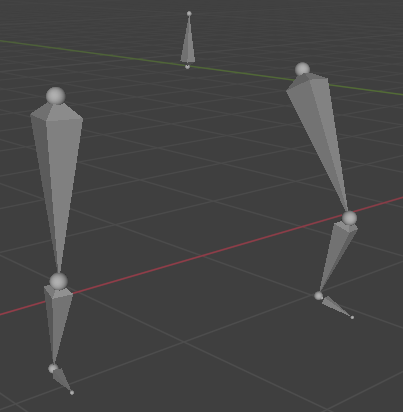
\includegraphics[width=6cm]{figure/piattoRig.png}
     \caption{Rig Umanoide} \label{fig:scheletro}
\end{center}
\end{figure}

L'approccio adottato rappresenta una versione semplificata dei metodi di rigging automatico più avanzati, traducendo in una procedura pratica alcuni dei principi teorici descritti nel capitolo precedente. Pur non implementando algoritmi di previsioni basati su modelli neurali o processi autoregressivi, lo script sviluppato in Blender consente di ottenere una \textbf{configurazione scheletrica adattativa}, riducendo in modo significativo i tempi di preparazione del rig e permettendo l'applicazione di animazione predefinite anche a modelli non organici.

\section{Implementazione dello skinning automatico in Blender}

Dopo la generazione automatica dello scheletro, la fase successiva del processo consiste nell'associazione tra la mesh nell'oggetto e la struttura scheletrica, ovvero lo \textbf{skinning}. Lo skinning rappresenta un passaggio fondamentale nel rigging, poichè determina in che modo i vertici della mesh si deformano in risposta ai movimenti delle ossa. L'obiettivo di questa fase è garantire una \textbf{deformazione realistica e coerente} dell'oggetto durante l'animazione, riducendo al minimo le distorsioni indesidetate.

Nel contesto di questo progetto, lo skinning è stato implementato in \textit{Blender} attraverso un \textbf{procedimento automatico}, con l'obiettivo di trasferire i pesi di influenza da un modello sorgente (un rig umanoide già animato) a un oggetto non organico, come un piatto o una tazzina dotati di gambe.

\subsection{Trasferimento pesi con algoritmi automatici}

Nel contesto della generazione automatica di rig, un aspetto fondamentale riguarda la previsone dei pesi di skinning, ovvero i coefficienti che definiscono l'influenza di ciascun osso sui vertici della mesh.
La determinazione di questi pesi è un problema di natura complessa, poichè implica la definizione di una matrice ad alta dimensionalità, in cui ogni riga corrisponde a un vertice della mesh e ogni colonna a un osso del rig. Nei modelli tridimensionali di alta risoluzione, tale matrice può raggiungere dimensioni considerevoli, rendendo il processo computazionalmente oneroso.

Le ricerche più recenti in ambito accademico hanno proposto approcci data-driven e basati su reti neurali autoregressive per stimare automaticamente tali pesi, integrando anche parametri aggiuntivi legali alle proprietà fisiche delle articolazioni (come rigità o gravità).
Questi metodi sfruttano meccanismi di cross-attention per modellare in modo efficiente la relazione tra la topologia dello scheletro e la geometria della mesh, migliorando la coerenza del movimento e la qualità della deformazione.

Nel caso di questo progetto, pur non adottando una soluzione di apprendimento automatico, lo \textit{skinning automatico} è stato implementato in Blender sequendo la stessa logica di corrispondenza tra ossa e vertici, ma attraverso uno script Python dedicato che trasferisce i pesi da un modello sorgente già pesato a un oggetto target.
Lo script esegue le seguenti operazioni principali:

\begin{enumerate}
    \item \textbf{Selezione delle ossa rilevanti}: vengono mantenuti esclusivamente i gruppi di pesi relativi alla parte inferiore del corpo, coerenti con lo scheletro generale nella fase precedente.
    
    \begin{minted}[fontsize=\small, bgcolor=lightgray, frame=lines, breaklines]{python}
    # Ossa da trasferire (bacino + gambe)
    # bones_to_keep: è la lista delle ossa rilevanti che verrano considerate durente il trasferimento
    bones_to_keep = [
    "mixamorig:Hips",
    "mixamorig:LeftUpLeg", "mixamorig:LeftLeg", "mixamorig:LeftFoot",
    "mixamorig:RightUpLeg", "mixamorig:RightLeg", "mixamorig:RightFoot"]
    \end{minted}

    \item \textbf{Copia dei gruppi di vertici}: per ogni osso selezionato, lo script copia i pesi corrispondenti a ciascun vertice, limitandosi ai valori effettivamente significativi (pesi maggiore di zero).

    \item \textbf{Creazione di nuovi gruppi di influenza}: per la mesh target, vengono generati automaticamente nuovi \textit{vertex group} corrispondenti alle ossa selezionate, garantendo la compatibilità con il rig del nuovo modello.
\end{enumerate}

\paragraph{Estratto del codice Python}

Un frammento rappresentativo dello script utilizzato in Blender mostra la copia dei gruppi di vertici e la creazione di nuovi gruppi di influenza

\begin{minted}[fontsize=\small, bgcolor=lightgray, frame=lines, breaklines]{python}
    plate = bpy.data.objects.get(PLATE_OBJ) # conserva tutti gli oggetti nella variabile globale
    source_mesh = bpy.data.objects.get(SOURCE_MESH)
    
    if not plate or not source_mesh:
        raise Exception("❌ Mesh non trovata!")
    
    # ================= TRASFERIMENTO PESI OTTIMIZZATO =================
    # Cancella eventuali vertex group già presenti sul piatto, che serve per evitare conflitti o 
    # duplicazioni dei pesi provenienti da precedenti tentativi di rigging
    plate.vertex_groups.clear()
    
    # Copia solo i gruppi delle ossa selezionate
    for vg in source_mesh.vertex_groups:
        if vg.name in bones_to_keep:
            # crea un nuovo gruppo di vertici sulla mesh del piatto
            new_vg = plate.vertex_groups.new(name=vg.name)
            # scorre tutti i vertici della mesh sorgente
            for i, v in enumerate(source_mesh.data.vertices):
                try:
                    w = vg.weight(i)
                    if w > 0.0:  # copia solo pesi maggiori di zero, che il vertice è influenzato
                                 # da quell'osso
                        new_vg.add([i], w, 'REPLACE') # aggiungi quel peso al corrispondente vertice
                                                      # della mesh targata
                except RuntimeError:
                    pass  # vertice non presente nel gruppo
\end{minted}

Questo frammento mostra come il sistema filtri automaticamente i pesi pertinenti a li assegni ai vertici correspondenti del nuovo modello. Il risultato è una \textbf{mappatura coerente tra ossa e mesh}, che consente di preservare la qualità delle deformazioni anche in presenza di una topologia differenti tra i due oggetti.

\begin{figure}[H]
\begin{center}
     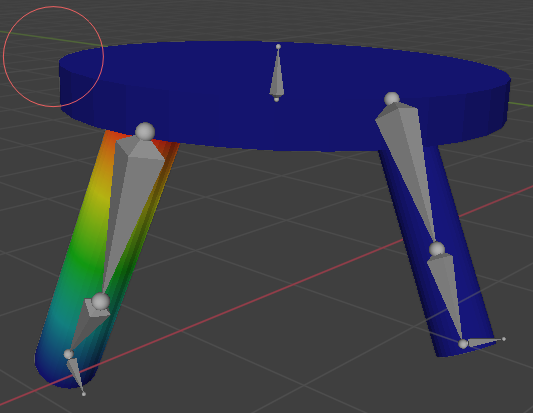
\includegraphics[width=6cm]{figure/pesi.png}
     \caption{Pesi assegnati alla mesh} \label{fig:scheletro}
\end{center}
\end{figure}

\subsection{Collegamento mesh-scheletro e gestione delle deformazioni}
Dopo il trasferimento dei pesi, la mesh viene collegata al rig mediante un modificatore di tipo \textit{Armature}, che permette a Blender di calcolare in tempo reale la deformazione dei vertici in base ai movimenti delle ossa.
Questo collegamento è del tutto automatico e viene completato senza intervento manuale, risultando in un processo di skinning completamente automatizzato.

L'efficacia del metodo è stata verifica attraverso test di animazione, applicando cicli di camminata e movimenti dinamici. I risultati mostrano che la deformazione delle gambe avviene in maniera stabile e coerente, con una buona trasmissione del movimento anche su modelli privi di articolazioni naturali.

\section{Retargeting dell'animazione}

Dopo la fase di rigging e di skinning automatico, in cui è stato generato e collegato lo scheletro al modello tridimensionale del piatto, la fase successiva ha riguardato l'\textbf{applicazione del movimento animato}.
In particolare, l'obiettivo è stato quello di \textbf{trasferire un'animazione umanoide preesistente}, proveniente da una sorgente esterna (come Mixamo), al modello personalizzato realizzato in Blender.

Questa operazione, nota come \textbf{retargeting dell'animazione}, consiste nel mappare i movimenti di un rig sorgente su un rig di destinazione avente una struttura scheletrica diversa, ma compatibile a livello gerarchico.
Nel contesto di questo lavoro, il retargeting ha permesso di riutilizzare animazioni di camminata o corsa tipiche di personaggi umanoidi per animare oggetti non convenzionati, come il \textit{piatto} o la \textit{tazzina con gambe}, generando un effetto dinamico coerente senza dever ricorrere a un'animazione manuale.

Il processo è stato sviluppato interamente in \textbf{Blender}, attraverso \textbf{script Python dedicati}, che automatizzano la fase di assegnazione dei vincoli di trasformazione tra rig sorgente e rig target. Questa automazione ha reso possibile un trasferimento accurato delle animazioni anche in presenza di differenze morfologiche significative tra i modelli, mantenendo la coerenza strutturale e la stabilità del movimento.

\subsection{Trasferimento di animazioni umanoidi agli oggetti}

Per permettere al modello non antropomorfo di riprodurre i movimenti di un rig umanoide (nel caso specifico, un'animazione di camminata proveniente da Mixamo), è stato realizzato un sistema di \textbf{retargeting automatico} all'interno di Blender tramite script Python.

L'obiettivo è mappare le ossa del rig sorgente (umanoide) su quelle di rig target (nel nostro caso il \textit{PiattoRig}), trasferendo posizione e rotazione delle articolazioni principali. Questo processo è stato implementato utilizzando \textbf{vincoli di trasformazione} (constraints) che permettono di copiare in tempo reale i movimenti del rig originale.

In particolare, per ciascun osso del rig del piatto, lo script aggiunge vincoli principali:

\begin{itemize}
    \item \textbf{Copy Location}, per copiare la posizione locale dell'osso corrispondente;
    \item \textbf{Copy Rotation}, per copiare la rotazione, mantenendo la coerenza con il sistema di coordinate locale.
\end{itemize}

\begin{figure}[H]
\begin{center}
     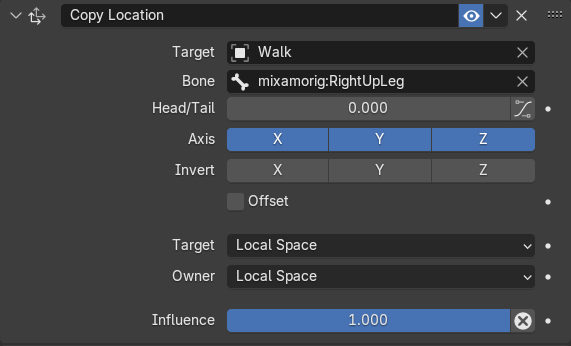
\includegraphics[width=10cm]{figure/copy.png}
     \caption{Vincoli Copy Location su Blender} 
     \label{fig:cop}
\end{center}
\end{figure}

L'approccio consente di sincronizzare i movimenti dell'intero rig, evitando la necessità di keyframe manuali o conversioni di animazioni tra sistemi scheletrici differenti. Un frammento esemplificativo del codice implementato è mostrato di seguito: 

\begin{minted}[fontsize=\small, bgcolor=lightgray, frame=lines]{python}
    for bone in target.pose.bones:
    src_bone = source.pose.bones.get(bone.name)
    if not src_bone:
        continue

    c_loc = bone.constraints.new(type='COPY_LOCATION')
    c_loc.target = source
    c_loc.subtarget = bone.name
    c_loc.owner_space = 'LOCAL'
    c_loc.target_space = 'LOCAL'

    c_rot = bone.constraints.new(type='COPY_ROTATION')
    c_rot.target = source
    c_rot.subtarget = bone.name
    c_rot.owner_space = 'LOCAL'
    c_rot.target_space = 'LOCAL'
\end{minted}

Questo frammento mostra la parte centrale dello script, in cui ad ogni osso viene assegnata una relazione diretta di copia di posizione e rotazione rispetto all'omologo del rig sorgente. Il risultato è un trasferimento fedele del movimento, applicato anche a oggetti con una morfologia completamente diversa da quella del modello originale.

\subsection{Gestione del movimento coerente (root motion o offset spaziali)}

Per garantire che l'oggetto animato mantenga un movimento coerente nello spazio, è stata introdotta una seconda fase di \textbf{controllo del root motion}, ovvero della traslazione globale del rig.

Il problema principale riscontrato riguarda l'osso radice (\textit{mixamorig:Hips}), che un rig umanoide controlla lo spostamento complessivo del corpo. Nel caso di un oggetto statico come il piatto, la riproduzione diretta di tale movimento avrebbe causato uno spostamento dell'intero modello lungo l'asse verticale.

Per risolvere questo problema, è stato utilizzato un secondo script che gestisce selettivamente il trasferimento delle trasformazioni, limitando il movimento all'asse orizontale (X e Y) e impedendo la traslazione lungo l'asse Z. L'estratto seguente illustra questa logica:

\begin{minted}[fontsize=\small, bgcolor=lightgray, frame=lines]{python}
    hips = target.pose.bones.get("mixamorig:Hips")
    if hips:
        c_loc = hips.constraints.new(type='COPY_LOCATION')
        c_loc.target = source
        c_loc.subtarget = "mixamorig:Hips"
        c_loc.owner_space = 'WORLD'
        c_loc.target_space = 'WORLD'
        c_loc.use_z = False  # non copiare l'altezza (Z)
    
        c_rot = hips.constraints.new(type='COPY_ROTATION')
        c_rot.target = source
        c_rot.subtarget = "mixamorig:Hips"
\end{minted}

Questa configurazione consente di preservare il \textbf{movimento orizzontale} del rig, mantenendo però fisso il punto di contatto del modello con il suolo. Il risultato è un'animazione fluida e coerente, dove il piatto segue la dinamica della camminata umanoide senza perdere l'allineamento spaziale.

\section{Analisi dei risultati}
\subsection{Valutazione visiva}

La valutazione qualitativa del modello animato si è concentrata principalmente sulla stabilità strutturale durante il movimento e sulla presenza di eventuali deformazioni anomale nella mesh (piatto e tazzina).
L'osservazione dei frame chiave ha permesso di verificare:

\begin{itemize}
    \item corretta risposta delle gambe alle rotazioni dei giunti.
    \item assenza di deformazioni non desiderate nel piatto e nella tazzina
    \item coerenza del movimento rispetto all'animazione sorgente
\end{itemize}

\subsection{Prestazioni}

Le prestazioni sono state analizzate considerando:

\begin{itemize}
    \item \textbf{FPS medi} durante la riproduzione dell'animazione
    \item \textbf{tempi di esecuzione} degli script di generazione dello scheletro e trasferimenti dei pesi.
    \item impatto delle operazioni di rigginge retargeting sulla scena di Blender
\end{itemize}
    
L'intera procedura si è dimostrata efficiente per modelli complessità ridotta come quelli considerati, garatendo un'interazione fluida e un processo automatizzato rapido.

\subsection{Limite tecnici e problematiche}

Nonostante i risultati complessivamente soddisfacenti, sono emerse alcune limitazioni:

\begin{itemize}
    \item lo scheletro generato replica solo in parte la struttura umana e non segue completamente le logiche generative dei modelli autoregressivi come UniRig;
    \item il trasferimento dei pesi basato su copia diretta da un modello umanoide può generare zone con pesi approssimativi;
    \item il retargeting richiede un allineamento iniziale accurato delle ossa e può produrre movimenti innaturali in assenza di vincoli aggiuntivi;
    \item il modello non implementa uno skinning automatico predittivo, come mostrato nella letteratura recente, ma una variante semplificata basata sul trasferimento pesi.
\end{itemize}






    

